\subsubsection*{Zadanie~3.123.}
\begin{figure}[H]
    \centering
    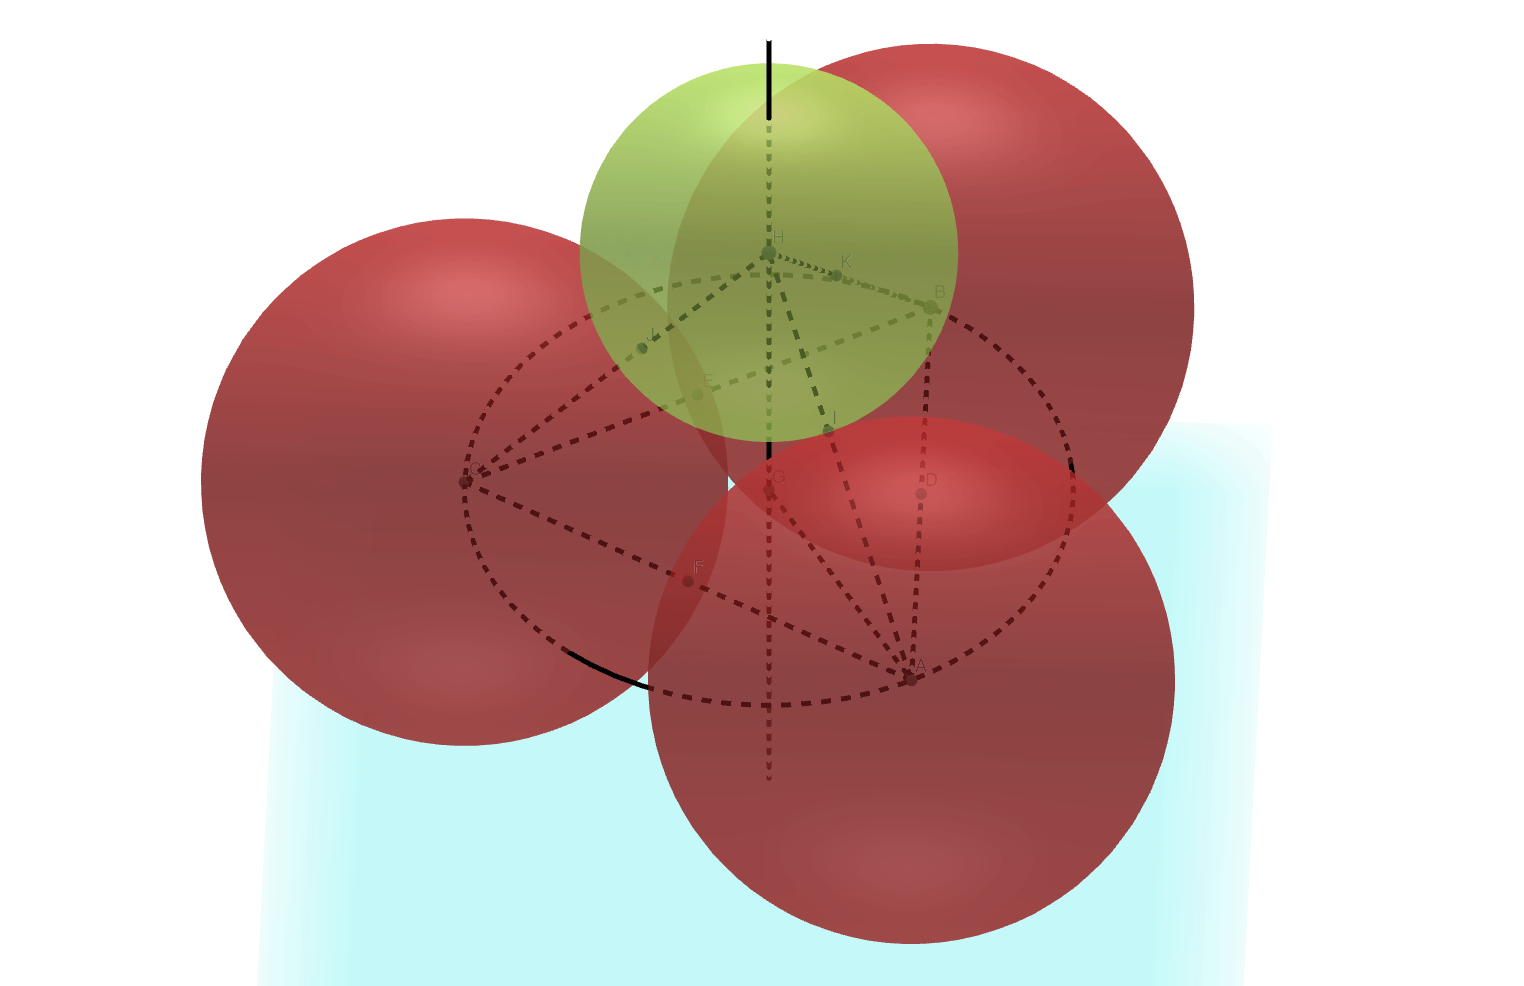
\includegraphics[width=\textwidth]{img/2021_02_24/123/space.png}
\end{figure}
Na początek obliczmy odległość środka czwartej kuli od stołu, później wystarczy dodać do tego \(r\). Zauważmy, że ponieważ trzy kule tworzące podstawę piramidy są identyczne, to ich środki, czyli punkty \(A\), \(B\), \(C\), wyznaczają wierzchołki trójkąta równobocznego o~boku \(2R\) w~płaszczyźnie równoległej do stołu i~odległej od niego o~\(R\). Ponieważ środek czwartej kuli jest równo odległy od środków pozostałych (dokładnie o~\(r + R\)) to musi leżeć na osi prostopadłej do płaszczyzny trójkąta \(\triangle{ABC}\) i~przechodzącej przez środek okręgu opisanego na nim. Jeśli oznaczymy środek czwartej kuli przez \(H\), a~środek okręgu opisanego na \(\triangle{ABC}\) przez \(G\), to \(\triangle{AGH}\) jest prostokątny. Z~własności trójkąta równobocznego wiemy, że
\begin{equation*}
    AG = \frac{2\sqrt{3}R}{3}
\end{equation*}
Możemy teraz wyliczyć z~twierdzenia Pitagorasa:
\begin{equation*}
    GH
    = \sqrt{AH^2 - AG^2}
    = \sqrt{\pars{R + r}^2 - \pars{\frac{2\sqrt{3}R}{3}}^2}
    = \sqrt{R^2 + 2Rr + r^2 - \frac{4R^2}{3}}
    = \sqrt{2Rr + r^2 - \frac{R^2}{3}}
\end{equation*}
Do tak wyliczonej odległości wystarczy dodać odległość punktu \(G\) od stołu oraz wspomnianą już długość promienia czwartej kuli. Zatem największa odległość punktu czwartej kuli od stołu wynosi
\begin{equation*}
    d = \sqrt{2Rr + r^2 - \frac{R^2}{3}} + R + r
\end{equation*}
\subsubsection*{Zadanie~3.124.}
\begin{mathfigure*}
    \coordinate (A) at (-4, -0.8);
    \coordinate (Bprime) at (2, -0.8);
    \coordinate (C) at (4, 0.8);
    \coordinate (Dprime) at (-2, 0.8);
    \coordinate (Aprime) at (-4, 5.2);
    \coordinate (B) at (2, 5.2);
    \coordinate (Cprime) at (4, 6.8);
    \coordinate (D) at (-2, 6.8);
    \coordinate (S) at ($(A)!0.5!(C)$);
    \coordinate (T) at ($(B)!0.5!(D)$);
    \coordinate (Q) at ($(A)!0.5!(Cprime)$);
    \draw (Q) circle[radius=\fpeval{0.85*sqrt(3)}];
    \draw (Q) circle[radius=\fpeval{3.21*sqrt(3)}];
    \draw[rotate=10] (S) ellipse (4.1 and 1.3);
    \draw[rotate=10] (T) ellipse (4.1 and 1.3);
    \draw[dashed] (A) -- (Bprime) -- (C);
    \draw[dotted] (C) -- (Dprime) -- (A);
    \draw[dotted] (D) -- (Dprime);
    \draw[Orange] (A) -- (B) -- (C) -- cycle;
    \draw[Orange] (B) -- (D);
    \draw[Orange, dashed] (C) -- (D) -- (A);
    \draw[dashed] (Aprime) -- (B) -- (Cprime) -- (D) -- cycle;
    \draw[dashed] (A) -- (Aprime);
    \draw[dashed] (B) -- (Bprime);
    \draw[dashed] (C) -- (Cprime);
\end{mathfigure*}
Środek sześcianu opisanego na czworościanie foremnym jest środkiem obydwu kul. Skoro przekątna ściany sześcianu ma długość \(a\), to~krawędź sześcianu ma długość \(\frac{a\sqrt{2}}{2}\).
\begin{equation*}
    \frac{V}{v}
    = \frac{\cancel{\frac{4}{3}\pi} R^3}{\cancel{\frac{4}{3}\pi} r^3}
    = \pars{\frac{R}{r}}^3
\end{equation*}
Połowa przekątnej sześcianu jest promieniem kuli opisanej. Natomiast promień kuli wpisanej w~czoworościan stanowi \(\frac{1}{4}\) połowy przekątnej, czyli \(\frac{1}{3}\) promienia kuli opisanej. Zatem
\begin{gather*}
    \frac{R}{r} = 3\\
    \frac{V}{v} = \pars{\frac{R}{r}}^3 = 3^3 = 27
\end{gather*}
